\chapter{Background and Related Technologies}
\label{chap:background}

The Keystone framework is founded on the RISC-V instruction set architecture (ISA), which provides a compelling platform for secure system design due to its open specification and extensible modularity~\cite{Lee2019,Lee2019}. Unlike traditional ISAs governed by proprietary vendors, RISC-V fosters a collaborative ecosystem that supports community-driven enhancements and custom extensions. This openness uniquely positions RISC-V as a prime candidate for trusted computing research and development~\cite{Survey2023}. Furthermore, its well-defined privilege model facilitates the construction of robust isolation mechanisms, which are essential for implementing Trusted Execution Environments (TEEs).\footnote{For an in-depth exposition of RISC-V privilege modes and PMP, see the RISC-V Privilege Specification v1.10~\cite{keystone2025how}.}

RISC-V specifies three hierarchical privilege levels: user mode (U-mode), supervisor mode (S-mode), and machine mode (M-mode). M-mode operates with the highest privilege and possesses unrestricted access to hardware resources, managing critical functions such as interrupt handling, exception processing, and physical memory protection~\cite{Lee2019}. Keystone capitalizes on this privilege hierarchy by situating its Security Monitor (SM)—the core Trusted Computing Base (TCB)—within M-mode. The SM is responsible for managing enclaves, enforcing strict memory isolation, and mediating access to sensitive operations. By anchoring the TCB at this highest privilege level, Keystone minimizes the trusted surface exposed to potential attackers.

A key hardware feature leveraged by Keystone is the Physical Memory Protection (PMP) unit, introduced in the RISC-V Privilege Specification v1.10. PMP empowers M-mode software to define fine-grained access permissions for physical memory regions, specifying which lower privilege levels (U and S) may read, write, or execute code therein~\cite{keystone2025how}. This hardware-enforced mechanism forms the cornerstone of Keystone’s memory isolation strategy. Each enclave is assigned a dedicated, PMP-protected memory region that remains inaccessible to the host OS or unauthorized software, guaranteeing strong confidentiality and integrity guarantees enforced at the hardware level~\cite{Lee2019}.

In addition to PMP, RISC-V’s flexible trap and exception handling model enables M-mode to intercept all traps while optionally delegating certain classes, such as system calls and page faults, to S-mode for efficiency~\cite{Lee2019}. This delegation mechanism facilitates cooperation between enclave runtimes and the host OS for memory management without compromising enclave boundaries. Keystone utilizes the RISC-V Memory Management Unit (MMU) to support private virtual address spaces per enclave, further fortified by PMP protections against unauthorized access or tampering~\cite{Lee2019}.

Notably, the Keystone Security Monitor is implemented in C using standard programming toolchains, which enhances maintainability, auditability, and formal verification potential. This contrasts with fixed-function microcode or proprietary firmware that is often opaque and difficult to analyze, thus bolstering Keystone’s transparency and security assurance~\cite{Lee2019}.

Together, the RISC-V privilege hierarchy, PMP, trap delegation, and extensibility create a robust substrate for implementing flexible, open, and secure TEEs. Keystone exploits these architectural advantages to deliver a customizable and transparent enclave platform aligned with the open philosophy of RISC-V~\cite{Survey2023}.

\section{Trusted Execution Environments}

Trusted Execution Environments (TEEs) are specialized hardware-assisted secure computing architectures designed to provide strong confidentiality and integrity guarantees for code and data, even in the presence of compromised system software~\cite{Survey2023,suzaki2021tsperf}. By establishing isolated execution contexts—often termed enclaves—TEEs protect sensitive computations through a combination of hardware-enforced isolation and minimal trusted software components.

A TEE effectively partitions system resources such as CPU registers, memory, and I/O peripherals, restricting access exclusively to trusted enclave applications. This isolation is enforced by the processor’s privilege levels, memory protection units, or dedicated security monitors, thereby preventing unauthorized entities—including kernel-level malware or user-space adversaries—from accessing or manipulating enclave data~\cite{brasser2020enclave}.

Security in TEEs hinges on minimizing the Trusted Computing Base (TCB), which encompasses all components that must be trusted for correct and secure operation. A smaller TCB reduces the risk of vulnerabilities and facilitates formal verification and security audits~\cite{Lee2019,Survey2023}. Modern TEEs strive to encapsulate only essential components within the TCB, balancing security with functionality.

Commercially dominant TEE solutions include Intel Software Guard Extensions (SGX) and ARM TrustZone. Intel SGX enables enclave creation at user privilege levels, employing hardware-enforced memory encryption and access controls~\cite{costan2016intel}. ARM TrustZone employs a split-world model that partitions processor execution into secure and normal worlds, with transitions mediated by secure monitor calls~\cite{yan2018trustzone}. These architectural designs are illustrated in Figure~\ref{fig:tee-architectures}, which compares TrustZone's dual-world architecture (Figure~\ref{fig:trustzone}) with SGX's Enclave Page Cache memory model (Figure~\ref{fig:sgx-epc}). Despite their widespread deployment, these architectures suffer from proprietary designs and limited transparency, which constrain their flexibility for academic research and system-level innovation.

\begin{figure}[htbp]
\centering
\begin{subfigure}[b]{0.48\linewidth}
  \centering
  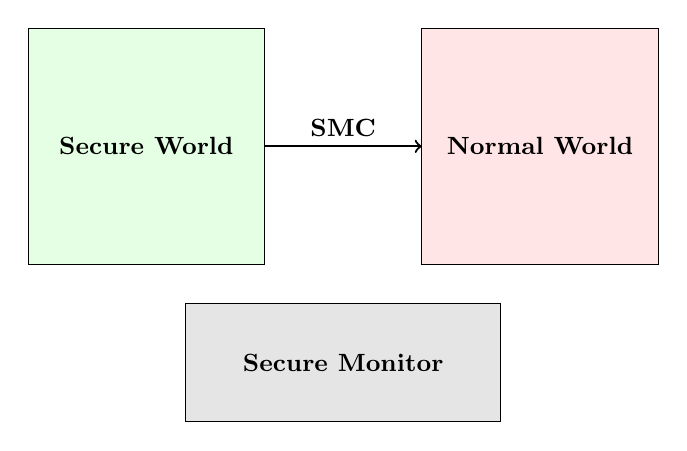
\begin{tikzpicture}[font=\small]
    \draw[fill=green!10] (0,2) rectangle (3,5) node[midway]{\textbf{Secure World}};
    \draw[fill=red!10] (5,2) rectangle (8,5) node[midway]{\textbf{Normal World}};
    \draw[fill=gray!20] (2,0) rectangle (6,1.5) node[midway]{\textbf{Secure Monitor}};
    \draw[->,thick] (3,3.5) -- (5,3.5) node[midway,above]{\textbf{SMC}};
  \end{tikzpicture}
  \caption{TrustZone's dual-world architecture with SMC-managed transitions.}
  \label{fig:trustzone}
\end{subfigure}
\hfill
\begin{subfigure}[b]{0.48\linewidth}
  \centering
  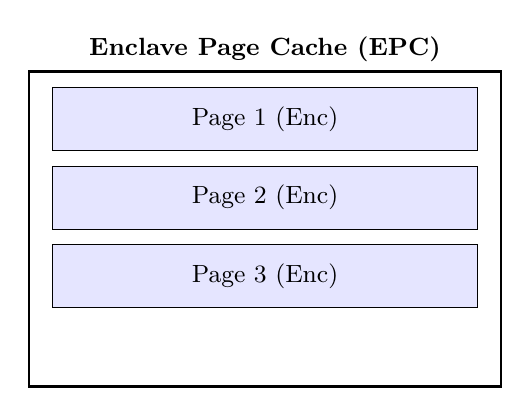
\begin{tikzpicture}[font=\small]
    \node[above] at (3,4) {\textbf{Enclave Page Cache (EPC)}};
    \draw[thick] (0,0) rectangle (6,4);

    \foreach \y/\label in {3.0/{Page 1 (Enc)}, 2.0/{Page 2 (Enc)}, 1.0/{Page 3 (Enc)}} {
      \fill[blue!10] (0.3,\y) rectangle (5.7,\y+0.8);
      \draw (0.3,\y) rectangle (5.7,\y+0.8) node[midway]{\label};
    }
  \end{tikzpicture}
  \caption{Intel SGX enclaves mapped to encrypted pages inside the EPC.}
  \label{fig:sgx-epc}
\end{subfigure}
\caption{Comparison of two TEE memory architectures: (a) ARM TrustZone split-world and (b) Intel SGX EPC memory model.}
\label{fig:tee-architectures}
\end{figure}

In contrast, open-source TEE frameworks such as Keystone have emerged to address these limitations by leveraging the open, modular RISC-V ISA~\cite{Lee2019}. The modularity and openness of RISC-V facilitate the design of TEEs that are both highly configurable and more transparent, fostering security research and experimentation~\cite{Survey2023}. A central architectural principle of TEEs, exemplified by Keystone, is privilege separation: executing the TCB in the highest privilege mode (M-mode in RISC-V) while relegating untrusted software to lower privilege levels. This design enforces strict isolation policies, preventing untrusted software from compromising enclave security~\cite{Lee2019}.
Table~\ref{tab:tee-comparison} summarizes key architectural and design distinctions between Intel SGX, ARM TrustZone, and Keystone.

\begin{table}[htbp]
\centering
\caption{Comparison of three TEE implementations.}
\label{tab:tee-comparison}
\small
%\renewcommand{\arraystretch}{1.2}
\begin{tabular}{@{}p{3cm}p{2.5cm}p{2.5cm}p{2.5cm}@{}}
\toprule
\textbf{Feature} & \textbf{Intel SGX} & \textbf{ARM TrustZone} & \textbf{Keystone} \\
\midrule
Privilege Model & Ring 3 enclaves & Secure Monitor & M-mode TCB \\
Openness & Closed & Closed & Open \\
Use Cases & Cloud security & Mobile security & Research, IoT \\
Hardware Dependency & Intel CPUs & ARM SoCs & RISC-V \\
\bottomrule
\end{tabular}
\end{table}


By integrating privilege separation, hardware-enforced memory protections, and modular TCB design, TEEs provide a powerful framework for secure computation within adversarial environments. Keystone extends these foundational principles with openness and configurability, offering a valuable platform for both academic research and practical deployments of trusted computing technologies~\cite{suzaki2021tsperf}.


\section{Keystone Enclave Architecture}

Keystone is an open-source Trusted Execution Environment (TEE) framework built on the RISC-V architecture, designed to enable customizable, lightweight, and secure enclaves suitable for both research and deployment in resource-constrained or security-critical settings \cite{Lee2019}. The framework’s modular design emphasizes a minimal Trusted Computing Base (TCB), portability across diverse RISC-V platforms, and extensibility to accommodate advanced security features, reflecting a clean and flexible architectural philosophy.

Keystone leverages the multiple privilege modes defined by the RISC-V specification—user mode (U-mode), supervisor mode (S-mode), and machine mode (M-mode)—to enforce security policies effectively. At the core of Keystone’s TCB is the Security Monitor (SM), which executes in M-mode and holds exclusive authority over enclave lifecycle management, memory protection configuration, and access control enforcement. The SM uses RISC-V’s Physical Memory Protection (PMP) mechanism to isolate enclave memory regions dynamically, ensuring strict access controls during enclave execution \cite{Lee2019}.

A typical Keystone-enabled platform comprises RISC-V cores augmented with secure boot mechanisms, trusted entropy sources, and optionally, hardware accelerators for cryptographic functions or secure I/O. Importantly, Keystone does not require hardware beyond standard RISC-V compliance and PMP support, making it adaptable to implementations ranging from FPGA prototypes to silicon SoCs \cite{Lee2019}.

Each enclave in Keystone consists of two main software components: a user-level enclave application (eapp) containing application-specific logic, and a supervisor-level runtime (RT) providing essential operating system abstractions such as exception handling, system call services, and memory management. This layered approach reduces the complexity of enclave applications and provides a trusted runtime environment isolated from the untrusted operating system and other processes \cite{Lee2019}.

The enclave lifecycle is structured into three primary phases: creation, execution, and destruction. During creation, the SM validates and locks the enclave’s memory layout—referred to as Enclave Page Memory (EPM)—with PMP to ensure confidentiality and integrity. During execution, the SM mediates context switches between the host and enclave, dynamically adjusting PMP to maintain isolation. Destruction securely erases enclave memory to prevent any residual data leakage \cite{Lee2019}. Keystone also supports optional features such as remote attestation, allowing external verifiers to authenticate enclave state prior to provisioning sensitive data, and can be extended for secure I/O and cryptographic acceleration.
Figure~\ref{fig:keystone_grouped} illustrates the Keystone enclave design. Specifically, Figure~\ref{fig:keystone_overview} shows the architectural components, including the Security Monitor, enclave runtime, and the RISC-V privilege hierarchy. Figure~\ref{fig:enclave_lifecycle} depicts the enclave lifecycle phases: creation, execution, and destruction.

\begin{figure}[htbp]
\centering
\begin{subfigure}[b]{0.9\linewidth}
    \centering
    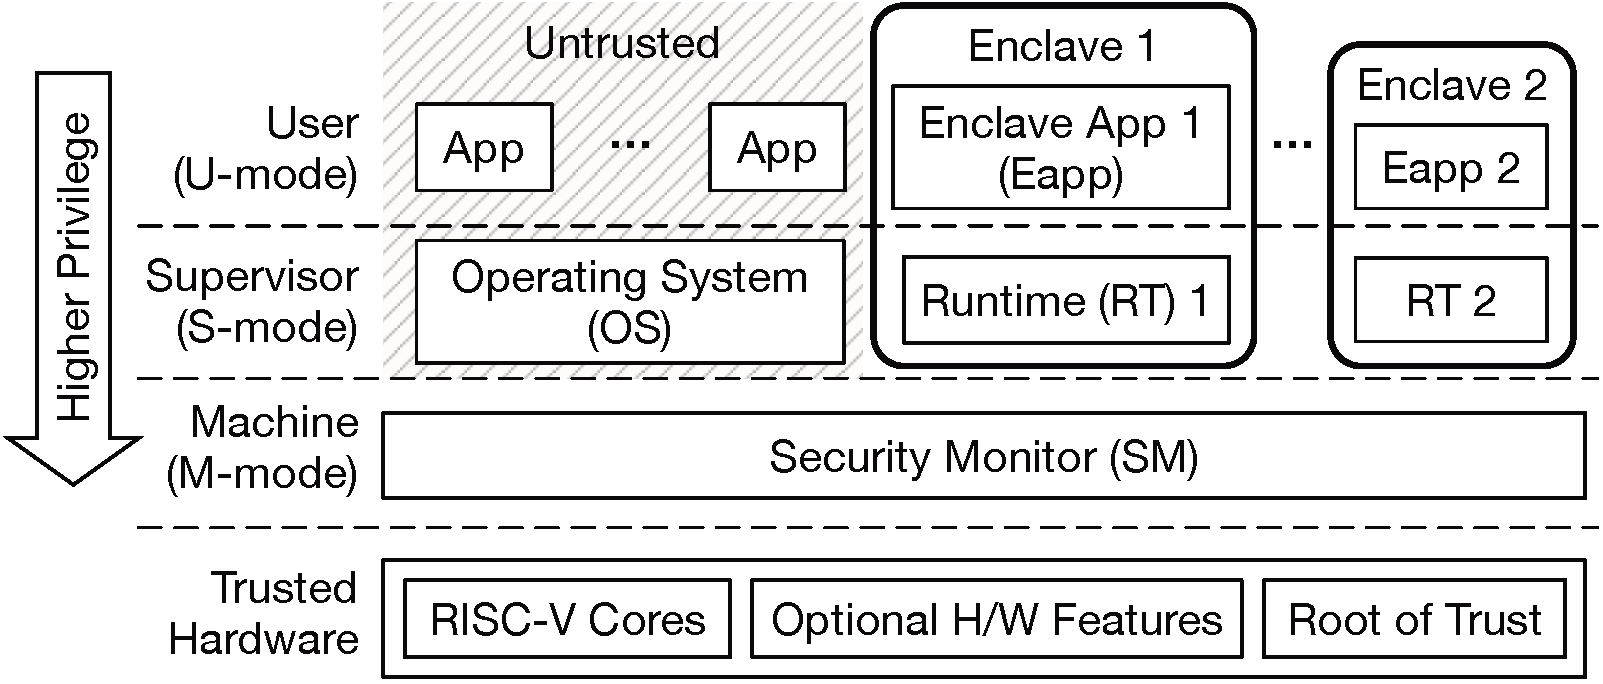
\includegraphics[width=\linewidth]{figures/keystone_overview.png}
    \caption{Keystone architecture showing components such as the Security Monitor, enclave runtime, and the privilege hierarchy.}
    \label{fig:keystone_overview}
\end{subfigure}

\vspace{0.5cm}

\begin{subfigure}[b]{0.9\linewidth}
    \centering
    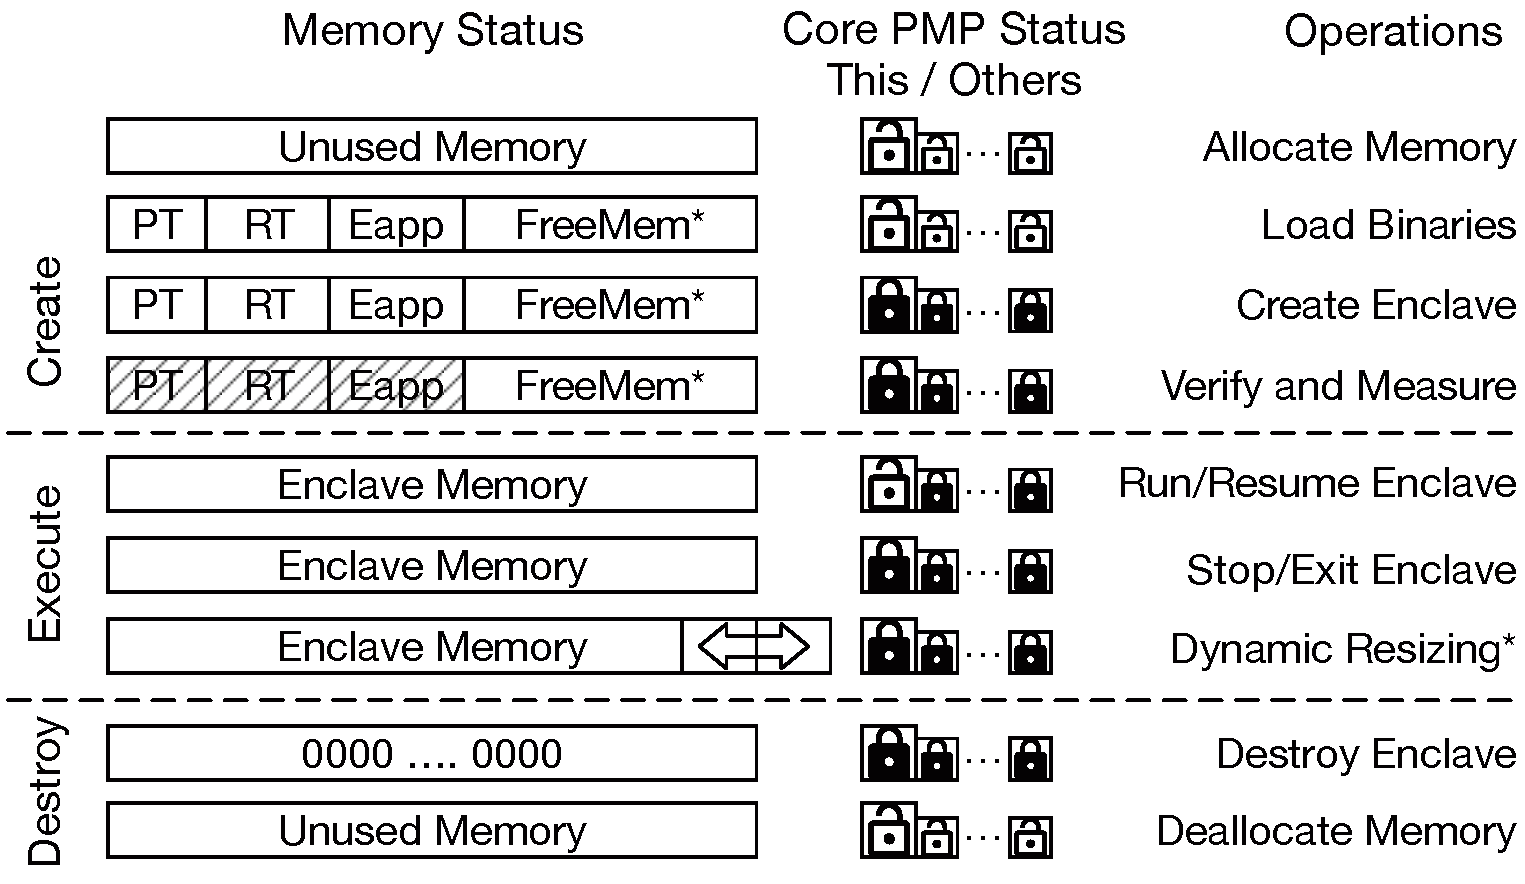
\includegraphics[width=\linewidth]{figures/enclave_lifecycle.png}
    \caption{Lifecycle of a Keystone enclave: creation, execution, and destruction phases.}
    \label{fig:enclave_lifecycle}
\end{subfigure}

\caption{Overview of the Keystone architecture and its enclave lifecycle.}
\label{fig:keystone_grouped}
\end{figure}

Keystone’s modular and open framework leverages the openness of RISC-V to provide strong security guarantees while enabling flexibility for research and customization. Its minimal TCB, modular layering (Security Monitor, runtime, eapp), and standards-compliant interfaces make it an attractive platform for developing and evaluating secure applications on modern processors \cite{Lee2019}. 
To support secure communication and attestation, Keystone enclaves can integrate modern cryptographic primitives, including emerging post-quantum schemes such as Kyber.

\section{Physical Memory Protection (PMP) in RISC-V}
\label{sec:pmp}

Physical Memory Protection (PMP) is a hardware-level security mechanism defined by the RISC-V privileged architecture to provide fine-grained control over access permissions to physical memory regions. PMP plays a central role in enabling secure system software, particularly in contexts where memory isolation between privileged and unprivileged software is essential. It is a critical enabler for implementing secure environments such as hypervisors, operating system kernels, and Trusted Execution Environments (TEEs) without relying on traditional virtualization support~\cite{riscvprivspec}.

In RISC-V, the PMP mechanism is configured exclusively by machine-mode (M-mode) software—the most privileged execution level in the architecture—and applies access control policies to all lower-privileged software running in supervisor (S-mode) or user mode (U-mode). Each PMP entry defines a memory region along with a set of permissions (read, write, execute) and an addressing mode. The hardware enforces these permissions such that any access attempt by S-mode or U-mode software that violates a PMP rule results in a trap to M-mode. This mechanism ensures that M-mode retains full control over physical memory while being able to delegate controlled access to untrusted software layers~\cite{riscvprivspec,Lee2019}.
The basic hardware architecture of PMP within the RISC-V privilege hierarchy is illustrated in Figure~\ref{fig:pmp-arch}.

\begin{figure}[htbp]
\centering
\begin{tikzpicture}[node distance=2.5cm,>=Stealth]
\tikzstyle{block} = [draw, minimum width=3cm, minimum height=2cm, align=center, font=\small]

\node[block, fill=gray!10] (cpu) {CPU Core\\\footnotesize Modes: M / S / U};
\node[block, fill=gray!20, right=of cpu] (pmp) {PMP Unit};
\node[block, fill=gray!30, right=of pmp] (mem) {Physical Memory};

\draw[->, thick] (cpu.east) -- node[above]{\footnotesize Access Request} (pmp.west);
\draw[->, thick] (pmp.east) -- node[above]{\footnotesize Permission Check} (mem.west);
\end{tikzpicture}
\caption{PMP hardware architecture in the RISC‑V privilege hierarchy. Memory accesses from the CPU are filtered through PMP entries to enforce physical memory protection.}
\label{fig:pmp-arch}
\end{figure}

A typical RISC-V core supports a fixed number of PMP entries (commonly 8 or 16), each represented by two Control and Status Registers (CSRs): \texttt{pmpcfg} and \texttt{pmpaddr}. The \texttt{pmpcfg} register specifies the access permissions and address matching mode for each region, while \texttt{pmpaddr} defines the address bounds. RISC-V supports several region encoding modes:

\begin{itemize}
    \item \textbf{TOR (Top-of-Range):} Defines a region from the base address of the previous PMP entry up to the current address.
    \item \textbf{NAPOT (Naturally Aligned Power-Of-Two):} Encodes both the base and size in a single register, enabling efficient representation of power-of-two-sized regions.
    \item \textbf{NA4 (Naturally Aligned 4-byte):} Encodes a minimal 4-byte memory region.
\end{itemize}

The design of PMP aligns with the minimalist and modular philosophy of RISC-V. Unlike traditional memory protection mechanisms such as x86's segmentation or ARM's TrustZone Address Space Controller (TZASC), PMP is simple, deterministic, and free from microarchitectural complexity. Importantly, PMP operates at the physical memory level—independent of virtual memory or page tables—which makes it highly suitable for systems with limited resources or without Memory Management Units (MMUs)~\cite{riscvprivspec,Survey2023}.

In the context of TEEs such as the Keystone framework, PMP serves as the fundamental enforcement mechanism for enclave isolation. Keystone leverages PMP to assign a protected memory region, known as the Enclave Page Memory (EPM), to each enclave. This region is configured to be inaccessible to both the untrusted operating system (running in S-mode) and any other software outside the enclave context~\cite{Lee2019}. During enclave creation, the Keystone Security Monitor (SM)—executing in M-mode—programmatically sets PMP entries to lock the memory region associated with the enclave. The SM verifies the integrity of the enclave binary, computes its cryptographic hash, and sets up the memory layout in such a way that only the enclave code has access to its memory contents~\cite{Lee2019,keystone2025how}.
As shown in Figure~\ref{fig:pmp-keystone}, the PMP unit mediates memory access between the OS and the enclave to enforce isolation guarantees.

\begin{figure}[htbp]
\centering
\begin{tikzpicture}[node distance=2.8cm,>=Stealth]
\usetikzlibrary{positioning, backgrounds}
\tikzstyle{block} = [draw, minimum width=3cm, minimum height=1.5cm, font=\small]

% Main nodes
\node[block, fill=gray!10] (os) {OS (S-mode)};
\node[block, fill=gray!20, right=of os] (pmpunit) {PMP Unit};
\node[block, fill=gray!30, right=of pmpunit] (enclave) {Enclave (EPM)};

% Arrows
\draw[->, thick] (os.east) -- node[above]{\footnotesize Memory Access} (pmpunit.west);
\draw[->, thick] (pmpunit.east) -- node[above]{\footnotesize Filtered Access} (enclave.west);

% Context switch label (moved lower)
\node[below=1.8cm of pmpunit, font=\footnotesize, fill=white, inner sep=2pt, rounded corners=1pt, draw=gray!50] 
    {Context switch $\Rightarrow$ PMP reconfig};

% Background shading (after everything else)
\begin{scope}[on background layer]
  % Only OS is untrusted
  \fill[red!10, opacity=0.3] 
    ($(os.north west)+(-0.4,0.4)$) rectangle 
    ($(os.south east)+(0.4,-0.4)$);

  % PMP + Enclave are trusted
  \fill[green!10, opacity=0.3] 
    ($(pmpunit.north west)+(-0.4,0.4)$) rectangle 
    ($(enclave.south east)+(0.4,-0.4)$);
\end{scope}

% Trust domain labels (moved closer to diagram)
\node[below=0.8cm of os, font=\scriptsize, align=center, fill=white, inner sep=2pt, draw=gray!40, rounded corners=1pt] 
    {Untrusted domain};

\node[below=0.8cm of enclave, font=\scriptsize, align=center, fill=white, inner sep=2pt, draw=gray!40, rounded corners=1pt] 
    {Trusted enclave memory};

\end{tikzpicture}
\caption{PMP-enforced isolation of Keystone enclaves. PMP is reconfigured on each context switch to protect enclave memory from the untrusted OS.}
\label{fig:pmp-keystone}
\end{figure}


Furthermore, PMP entries are reconfigured dynamically during enclave context switches. For example, when the host operating system regains control, the PMP settings are altered to revoke access to the enclave’s memory. Conversely, when the enclave resumes execution, the SM reinstates its PMP region. This dynamic switching is essential to enforce temporal isolation and prevent time-of-check-to-time-of-use (TOCTTOU) vulnerabilities that may arise during state transitions~\cite{lee2022cerberus}.

Despite its utility, PMP has several practical limitations. The fixed number of PMP entries restricts the number of simultaneously protected regions, posing a challenge for complex systems with many isolated domains or subregions. Moreover, overlapping PMP regions are resolved based on entry priority (lower-numbered entries take precedence), requiring careful configuration to avoid inadvertent leaks or privilege escalations (see Figure~\ref{fig:pmp-priority})~\cite{riscvprivspec}.

\begin{figure}[htbp]
\centering
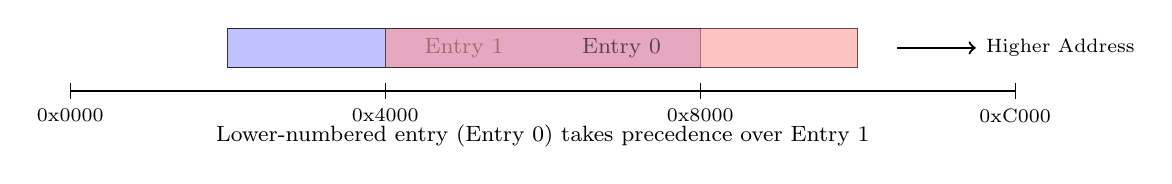
\begin{tikzpicture}
% Memory line
\draw[thick] (0,0) -- (12,0);

% Address labels
\foreach \x/\lbl in {0/0x0000, 4/0x4000, 8/0x8000, 12/0xC000} {
    \draw (\x,0.1) -- (\x,-0.1) node[below, font=\scriptsize] {\lbl};
}

% Entry regions
\draw[fill=blue!30, opacity=0.8] (2,0.3) rectangle (8,0.8)
    node[pos=.5, font=\footnotesize] {Entry 1};
\draw[fill=red!40, opacity=0.6] (4,0.3) rectangle (10,0.8)
    node[pos=.5, font=\footnotesize, text=black] {Entry 0};

% Priority indication
\draw[->, thick] (10.5,0.55) -- (11.5,0.55) node[right, font=\scriptsize] {Higher Address};
\node[below, font=\footnotesize] at (6,-0.3) {Lower-numbered entry (Entry 0) takes precedence over Entry 1};
\end{tikzpicture}
\caption{Overlapping PMP regions. When regions overlap, the lower-numbered PMP entry has priority.}
\label{fig:pmp-priority}
\end{figure}


Security researchers have explored various enhancements and formal models to increase the reliability and verifiability of PMP-based isolation. For example, Cerberus~\cite{lee2022cerberus} builds a formally verified memory-sharing abstraction over PMP to enable safe communication between enclaves and untrusted components. Similarly, HexBox~\cite{hexbox2018} leverages PMP for real-time embedded security by associating memory regions with specific control-flow paths in embedded firmware, demonstrating PMP's applicability beyond general-purpose computing.
Table~\ref{tab:pmp-limitations} summarizes key limitations in PMP and highlights recent research directions aimed at overcoming them.

\begin{table}[htbp]
\centering
\caption{Summary of PMP limitations and research‑driven enhancements.}
\label{tab:pmp-limitations}
\renewcommand{\arraystretch}{1.2}
\begin{tabular}{>{\raggedright}p{3cm} >{\raggedright}p{4cm} >{\raggedright\arraybackslash}p{5cm}}
\hline
\textbf{Limitation} & \textbf{Impact} & \textbf{Enhancement / Research} \\
\hline
Fixed \# entries & Limits scalability & Cerberus verified sharing \\
No dynamic resizing & Hard to adapt to workloads & Dynamic PMP proposals \\
Limited granularity & Coarse protection & Fine‑grained tagging \\
\hline
\end{tabular}
\end{table}

The role of PMP in Keystone exemplifies how low-complexity hardware primitives can be orchestrated by secure software layers to implement strong isolation guarantees. This synergy is particularly effective in the RISC-V ecosystem, where the open architecture allows deep customization, formal verification, and academic experimentation~\cite{Survey2023}. The combination of PMP, a secure boot mechanism, and a minimal TCB enables Keystone to enforce hardware-rooted enclave isolation without relying on opaque, vendor-specific extensions, setting it apart from alternatives like Intel SGX or ARM TrustZone~\cite{Lee2019,suzaki2021tsperf}.

Physical Memory Protection in RISC-V is a powerful, lightweight, and deterministic mechanism that underpins secure execution in many RISC-V-based platforms. Its integration into frameworks like Keystone enables transparent and verifiable enclave isolation while remaining suitable for constrained systems. As the RISC-V ecosystem continues to evolve, PMP will remain a fundamental building block for secure, open, and formally analyzable trusted computing platforms.

\section{Post-Quantum Cryptography: Kyber Algorithm}
\label{sec:kyber}

Kyber is a post-quantum key encapsulation mechanism (KEM) designed to remain secure against both classical and quantum adversaries. It is based on the hardness of the Module Learning With Errors (Module-LWE) problem, a structured lattice problem believed to be difficult to solve even with quantum algorithms \cite{kyber2021}. The algorithm has been selected by NIST for standardization in its post-quantum cryptography project, reflecting both its strong theoretical foundation and practical efficiency \cite{kyber2024}.

Kyber uses polynomial arithmetic in a modular ring to perform its cryptographic operations. It is based on the LPR encryption framework \cite{kyber2021}, which adapts the Learning With Errors (LWE) problem from integer vectors to more structured polynomial rings. This allows for faster computation and more compact key sizes compared to classical public-key systems.

Kyber supports three variants, each corresponding to a different level of security roughly equivalent to asymmetric encryption:

\begin{verbatim}
Kyber-512   → AES-128-level security
Kyber-768   → AES-192-level security (recommended)
Kyber-1024  → AES-256-level security
\end{verbatim}

These parameters determine the number of polynomials, noise levels, and compression factors used internally. Figure~\ref{fig:kyber_768} illustrates the Kyber-768 key exchange process, in which two parties derive a shared secret using public key encapsulation and decapsulation.

\begin{figure}[htbp]
\centering
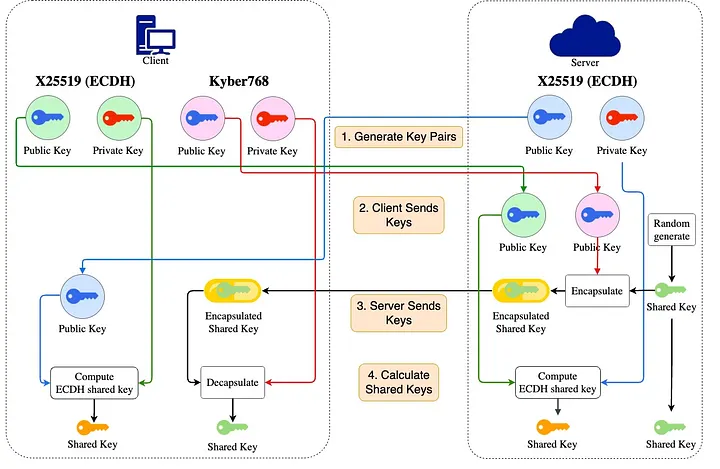
\includegraphics[width=0.9\linewidth]{figures/kyber_768.png}
\caption{Kyber-768 Key Exchange Algorithm \cite{Pathum_2025}}
\label{fig:kyber_768}
\end{figure}

Kyber exposes a compact and simple interface for use in protocols. Its API supports three core operations: key generation, encapsulation, and decapsulation, as shown in Listing~\ref{lst:kem_api}.

\begin{lstlisting}[style=kemstyle, caption={Kyber KEM API}, label={lst:kem_api}]
(pk, sk)    = KeyGen()           # Generate key pair
(ct, ss)    = Encapsulate(pk)    # Encrypt shared secret
ss          = Decapsulate(sk, ct) # Decrypt to recover secret
\end{lstlisting}

Compared to classical schemes like RSA, Kyber offers more compact key and ciphertext sizes at higher security levels. Table~\ref{tab:kyber_sizes} compares the relevant sizes in bytes for Kyber and RSA \cite{kyber2024}.

\begin{table}[h]
\centering
\caption{Key and Ciphertext Sizes (bytes)}
\label{tab:kyber_sizes}
\renewcommand{\arraystretch}{1.2}
\begin{tabular}{lccc}
\toprule
\textbf{Scheme} & \textbf{Private Key} & \textbf{Public Key} & \textbf{Ciphertext} \\
\midrule
Kyber-512 & 1632 & 800 & 768 \\
Kyber-768 & 2400 & 1184 & 1088 \\
Kyber-1024 & 3168 & 1568 & 1568 \\
RSA-3072 & 384 & 384 & 384 \\
RSA-15360 & 1920 & 1920 & 1920 \\
\bottomrule
\end{tabular}
\end{table}

The parameters that define Kyber’s security and performance are listed in Table~\ref{tab:kyber-params}. These include the polynomial degree, modulus, and bounds on the error distributions used to introduce noise in the ciphertexts \cite{kyber2021}.

\begin{table}[h]
\centering
\caption{Kyber Parameters}
\label{tab:kyber-params}
\renewcommand{\arraystretch}{1.2}
\begin{tabular}{ll}
\toprule
\textbf{Parameter} & \textbf{Description} \\
\midrule
$n = 256$ & Polynomial degree \\
$k \in \{2,3,4\}$ & Number of polynomials (varies by variant) \\
$q = 3329$ & Prime modulus for coefficients \\
$\eta_1, \eta_2$ & Noise bounds in key/ciphertext \\
$d_u, d_v$ & Compression factors \\
\bottomrule
\end{tabular}
\end{table}

Kyber has been optimized for modern platforms. Figure~\ref{fig:kyber_perf} shows benchmark cycle counts for each variant on an Intel Haswell CPU using AVX2 vector instructions \cite{kyber2024}. These results reflect Kyber’s suitability for high-performance and embedded applications alike.

\begin{figure}[h]
\centering
\begin{tikzpicture}
\begin{axis}[
    ybar,
    bar width=12pt,
    width=12cm,
    height=7cm,
    enlarge x limits=0.2,
    ylabel={Cycles},
    symbolic x coords={Kyber-512,Kyber-768,Kyber-1024},
    xtick=data,
    ymin=0,
    legend style={at={(0.5,-0.15)}, anchor=north, legend columns=-1},
    nodes near coords,
    every node near coord/.append style={
        font=\small,
        rotate=90,   % vertical labels
        anchor=west  % position so they sit neatly above bars
    },
    tick label style={font=\small},
    label style={font=\small},
    legend cell align={left},
    grid=major
]

% KeyGen
\addplot[
    pattern=north east lines,
    pattern color=black
] coordinates {
    (Kyber-512,33856) (Kyber-768,52732) (Kyber-1024,73544)
};

% Encaps
\addplot[
    pattern=dots,
    pattern color=black
] coordinates {
    (Kyber-512,45200) (Kyber-768,67624) (Kyber-1024,97324)
};

% Decaps
\addplot[
    pattern=crosshatch,
    pattern color=black
] coordinates {
    (Kyber-512,34572) (Kyber-768,53156) (Kyber-1024,79128)
};

\legend{KeyGen, Encaps, Decaps}
\end{axis}
\end{tikzpicture}
\caption{Kyber Performance on Haswell CPU (AVX2 Optimized)}
\label{fig:kyber_perf}
\end{figure}

For platforms that lack efficient SHAKE implementations, Kyber also offers a variant called \texttt{Kyber-90s}, which uses AES-256 and SHA2 instead. This allows faster execution on devices with AES hardware acceleration, such as many embedded and mobile processors \cite{kyber2024}.

Kyber has already been deployed in practice. Cloudflare integrated Kyber into its CIRCL library to support post-quantum TLS; Amazon added hybrid Kyber modes to its AWS Key Management Service; IBM deployed Kyber in a quantum-resistant tape storage system \cite{kyber2024}. These real-world uses demonstrate its maturity and readiness for deployment.

Thanks to its compact keys and efficient operations, Kyber is particularly well-suited for resource-constrained environments such as Trusted Execution Environments (TEEs). In this thesis, we evaluate the performance of Kyber within RISC-V-based enclaves and explore best practices for securely configuring post-quantum key exchange in such systems.

\section{Comparative Overview of TEE}
\label{sec:comparison_tees}

Keystone distinguishes itself from commercial Trusted Execution Environments—such as Intel SGX, ARM TrustZone, and AMD SEV—through its unique design choices, combining openness, modularity, and deep alignment with the RISC‑V ecosystem.

First and foremost, Keystone is fully open-source, enabling complete transparency and extensibility. This contrasts sharply with the proprietary nature of SGX, TrustZone, and SEV, which limits research innovation and system adaptability \cite{suzaki2021tsperf}. The open stance of Keystone allows researchers to inspect, customize, and formally verify its components, significantly reducing the Trusted Computing Base (TCB) compared to monolithic Secure World kernels or hardware-bound enclaves \cite{suzaki2021tsperf}. The estimated relative TCB sizes are shown in Figure~\ref{fig:tcb-size}, highlighting Keystone's minimal footprint.

\begin{figure}[htbp]
\centering
\begin{tikzpicture}
\begin{axis}[
    xbar,
    width=10cm, height=5cm,
    xmin=0, xmax=100,
    xlabel={Relative TCB size (\%)},
    symbolic y coords={SEV,SGX,TrustZone,Keystone},
    ytick=data,
    nodes near coords,
    every node near coord/.append style={font=\scriptsize},
    bar width=10pt
]
\addplot[pattern=north east lines] coordinates {(60,SEV) (50,SGX) (80,TrustZone) (20,Keystone)};
\end{axis}
\end{tikzpicture}
\caption{Estimated relative TCB sizes (illustrative).}
\label{fig:tcb-size}
\end{figure}

ARM TrustZone operates using a dual-world model: a Secure World and a Normal World, switching through secure monitor calls (SMCs). While effective, this design suffers from overhead due to frequent context switching and increased TCB complexity since the Secure World often incorporates a full OS stack (e.g., OP‑TEE) \cite{suzaki2021tsperf}. In contrast, Intel SGX allows enclave creation at user-level with encrypted memory regions but remains constrained by limited enclave size, single-mode operation, and dependency on Intel hardware, hindering portability and flexibility \cite{suzaki2021tsperf}. Figure~\ref{fig:ctx-overhead} compares the context switch latency across these systems, showing Keystone with the lowest overhead.

\begin{figure}[htbp]
\centering
\begin{tikzpicture}
\begin{axis}[
    ybar,
    symbolic x coords={TrustZone SMC,SGX ECALL,Keystone call},
    xtick=data,
    ylabel={Latency ($\mu$s)},
    ymin=0, ymax=12,
    nodes near coords,
    bar width=14pt
]
\addplot[pattern=dots] coordinates {(TrustZone SMC,10) (SGX ECALL,8) (Keystone call,3)};
\end{axis}
\end{tikzpicture}
\caption{Illustrative context switch latency across TEEs.}
\label{fig:ctx-overhead}
\end{figure}

Keystone effectively synthesizes the strengths of these platforms while avoiding their limitations. It supports dynamic enclave creation spanning both user and supervisor modes, with security ensured via low-overhead Physical Memory Protection (PMP) and a lightweight, verifiable Security Monitor operating in M-mode \cite{Lee2019}. This design offers richer enclave functionality with reduced complexity.

Empirical comparisons further highlight Keystone’s competitive performance. TS‑Perf, a systematic benchmarking framework, measured execution time across SGX, TrustZone, and RISC‑V Keystone using identical binaries and workloads (e.g., internal APIs, matrix operations, memory and storage access). It reports how architectural differences manifest in performance across ecosystems \cite{turn0search5}. As shown in Figure~\ref{fig:bench-compare}, Keystone achieves near-native performance on CPU-bound workloads and maintains a balanced profile across memory and I/O operations when compared to SGX and TrustZone.

The evolution of these TEEs over time is visualized in Figure~\ref{fig:tee-timeline}, placing Keystone's introduction in the broader historical context of trusted computing innovation.

Feature-wise, trusted computing surveys place Keystone in a distinct category: unlike SGX and SEV, which emphasize encryption and hardware-rooted attestation, Keystone enables both secure and flexible enclave configurations, attested through PMP and monitor mechanisms, and retains openness—making it uniquely suitable for research-oriented and evolving hardware/software environments \cite{turn0search9}. Table~\ref{tab:tee-features} summarizes key differences in TEE capabilities across Keystone, SGX, TrustZone, and SEV.

For these reasons, Keystone represents a promising alternative to closed-source TEEs, especially in academic and experimental contexts.


\begin{figure}[htbp]
\centering

% --- Benchmark Comparison Chart ---
\begin{subfigure}[b]{0.95\linewidth}
\centering
\begin{tikzpicture}
\begin{axis}[
    ybar,
    bar width=8pt,
    width=10cm, height=6cm,
    ymin=0, ymax=110,
    ylabel={Relative performance (\%)},
    symbolic x coords={CPU-bound,Memory-bound,I/O-bound},
    xtick=data,
    ymajorgrids,
    legend style={at={(0.5,-0.2)},anchor=north,legend columns=3}
]
\addplot[pattern=north east lines] coordinates {(CPU-bound,98) (Memory-bound,70) (I/O-bound,65)};
\addplot[pattern=dots] coordinates {(CPU-bound,100) (Memory-bound,50) (I/O-bound,55)};
\addplot[pattern=crosshatch] coordinates {(CPU-bound,95) (Memory-bound,60) (I/O-bound,50)};
\legend{Keystone, SGX, TrustZone}
\end{axis}
\end{tikzpicture}
\caption{Illustrative TS‑Perf-style benchmark comparison (REE = 100\%).}
\label{fig:bench-compare}
\end{subfigure}

\vspace{1em}

% --- Timeline ---
\begin{subfigure}[b]{0.95\linewidth}
\centering
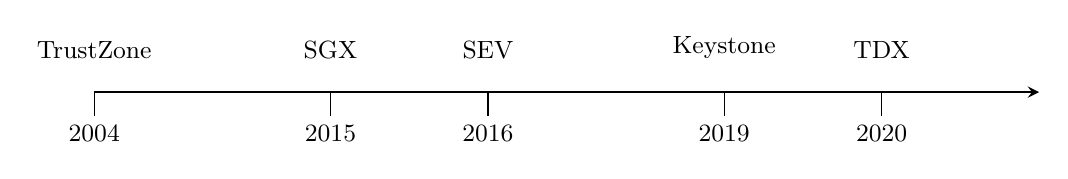
\begin{tikzpicture}[>=stealth, font=\small]
\draw[->, thick] (0,0) -- (12,0);
\foreach \x/\year/\name in {0/2004/TrustZone,3/2015/SGX,5/2016/SEV,8/2019/Keystone,10/2020/TDX} {
    \draw (\x,0) -- (\x,-0.3) node[below] {\year};
    \node[above=0.3cm] at (\x,0) {\name};
}
\end{tikzpicture}
\caption{Timeline of selected Trusted Execution Environment (TEE) introductions.}
\label{fig:tee-timeline}
\end{subfigure}

\caption{Performance, evolution, and feature comparison of major TEEs.}
\label{fig:tee-overview}
\end{figure}

\vspace{1em}

\begin{table}[htbp]
\centering
\caption{Feature comparison of major TEEs.}
\label{tab:tee-features}
\begin{tabular}{@{}lcccc@{}}
\toprule
\textbf{Feature} & \textbf{Keystone} & \textbf{SGX} & \textbf{TrustZone} & \textbf{SEV} \\
\midrule
Open Source & Yes & No & No & No \\
Dynamic Enclaves & Yes & No & Limited & No \\
Hardware Dependency & RISC-V & Intel & ARM & AMD \\
TCB Size & Low & Medium & High & Medium \\
Flexible Configurations & High & Low & Low & Medium \\
\bottomrule
\end{tabular}
\end{table}


\section{Performance Challenges in Secure Execution}

Trusted Execution Environments (TEEs) introduce strong isolation guarantees that are essential for secure computation, but these guarantees often come at the cost of non-negligible performance overheads. This performance degradation arises from several sources, including architectural constraints, software abstraction layers, and platform-specific implementation trade-offs. Understanding these performance characteristics is crucial to evaluating the practical deployment of TEEs, especially in scenarios requiring low latency or high throughput.

Compute-bound workloads tend to experience the least disruption from TEE isolation mechanisms. Operations such as arithmetic computations that remain within the processor’s execution pipeline typically show minimal slowdown. Empirical studies using TS-perf and Keystone’s own benchmarking tools (e.g., CoreMark and RV8) indicate that when enclave creation and destruction costs are excluded, the performance overhead of TEEs for CPU-intensive tasks is often below 1\%, with Intel SGX, ARM TrustZone, and RISC-V Keystone all exhibiting similar behavior \cite{suzaki2021tsperf,Lee2019}.

However, memory-bound applications face a very different scenario. Memory isolation mechanisms—particularly those involving encryption, cache partitioning, and page fault handling—can significantly impact runtime performance. For instance, in the Keystone framework, applications such as \texttt{miniz} and \texttt{aes} that utilize large memory footprints have shown over 100\% slowdown when cache partitioning is enabled, due to increased cache misses and eviction rates \cite{Lee2019}. Similarly, TS-perf benchmarks report an 11\% reduction in performance for ARM TrustZone under random memory access workloads, largely attributable to memory encryption and hierarchy constraints \cite{suzaki2021tsperf}. SGX-based systems experience a sharp decline in performance once the enclave's memory usage exceeds the size of the Enclave Page Cache (EPC), which triggers expensive paging behavior. This degradation is illustrated in Figure~\ref{fig:epc-cliff}, where performance drops dramatically beyond the 256~MB EPC boundary. This trend has been comprehensively documented by SGXGauge \cite{kumar2022sgxgauge}, with slowdown factors ranging from 1.2× up to 126× depending on the workload and hardware configuration \cite{akkram2020scientific}.

\begin{figure}[htbp]
\centering
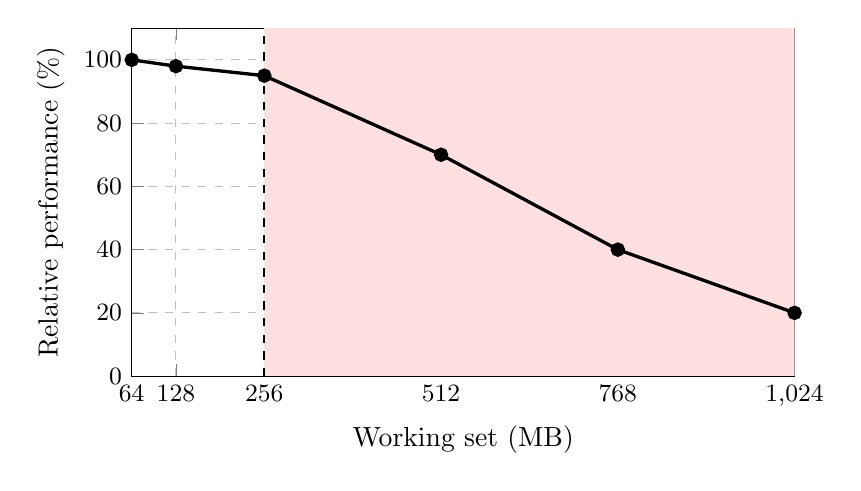
\begin{tikzpicture}
\begin{axis}[
    width=10cm, height=6cm,
    xlabel={Working set (MB)},
    ylabel={Relative performance (\%)},
    xmin=64, xmax=1024,
    ymin=0, ymax=110,
    xtick={64,128,256,512,768,1024},
    ytick={0,20,40,60,80,100},
    xmajorgrids, ymajorgrids, grid style=dashed,
    ticklabel style={font=\small}
]
% Shaded region beyond EPC size (example: 256 MB)
\path[fill=red!12, draw=none] (axis cs:256,0) rectangle (axis cs:1024,110);

% Performance curve (illustrative)
\addplot[black, very thick, mark=*, mark options={fill=black}] coordinates {
(64,100) (128,98) (256,95) (512,70) (768,40) (1024,20)
};

% EPC boundary
\addplot[dashed, black, thick] coordinates {(256,0) (256,110)};
\node[font=\footnotesize, fill=white, inner sep=1pt, anchor=south east]
    at (axis cs:256,110) {EPC boundary};

\end{axis}
\end{tikzpicture}
\caption{Performance drops sharply once the working set exceeds the protected memory size (shaded)}
\label{fig:epc-cliff}
\end{figure}


To address these performance issues, researchers have proposed alternative memory models that relax or restructure the traditional enclave-host memory boundaries. One such innovation is Elasticlave, a shared-memory model designed for enclaves that reduces isolation costs while preserving strong security properties. Elasticlave achieves an order of magnitude better performance compared to traditional spatial isolation models, with overheads as low as 10\% versus 100× to 1000× for spatially isolated configurations \cite{yu2022elasticlave}. Similarly, Eleos introduces self-paging within enclaves, allowing the enclave itself to manage virtual memory. This eliminates host OS involvement in page fault handling and mitigates context-switching and cache pollution overheads, resulting in significantly improved runtime efficiency \cite{orenbach2023eleos}. A related approach, Cerberus, applies formal methods to build a provably secure enclave memory-sharing model on Keystone. It enables safe data sharing with external components without compromising security, all while reducing redundancy and memory copying overheads \cite{lee2022cerberus}.

Input/output (I/O) operations also suffer substantial performance penalties in TEE contexts due to the need for secure copying and context switching. In Keystone, file I/O performance as measured using IOZone demonstrates a 36.2\% decrease in write throughput and a 40.9\% reduction in read throughput compared to execution in the Rich Execution Environment (REE). Repetitive operations, such as record rewriting, exhibit even greater overhead—up to 55.1\% \cite{Lee2019}. These results are visualized in Figure~\ref{fig:io-throughput}, which compares enclave and REE performance across several I/O workloads. Similar trends have been reported for other platforms; TS-perf reveals that both OP-TEE and SGX-based file operations incur high latency due to reliance on ECALLs and limited in-enclave storage APIs \cite{suzaki2021tsperf}.

\begin{figure}[htbp]
\centering
\begin{tikzpicture}
\begin{axis}[
    ybar,
    bar width=12pt,
    width=10cm, height=6cm,
    ymin=0, ymax=110,
    ylabel={Relative throughput (\%)},
    symbolic x coords={Write,Read,Rewrite},
    xtick=data,
    ymajorgrids, grid style=dashed,
    legend style={at={(0.5,-0.25)},anchor=north,legend columns=2, font=\small},
    pattern color=black,
    nodes near coords,
    every node near coord/.append style={font=\scriptsize}
]
% Enclave (throughput = 100 - slowdown)
\addplot[pattern=north east lines] coordinates {(Write,63.8) (Read,59.1) (Rewrite,44.9)};
% REE baseline
\addplot[pattern=vertical lines] coordinates {(Write,100) (Read,100) (Rewrite,100)};
\legend{Enclave,REE}
\end{axis}
\end{tikzpicture}
\caption{I/O throughput degradation in enclaves relative to REE: write (−36.2\%), read (−40.9\%), and record rewrite (−55.1\%).}
\label{fig:io-throughput}
\end{figure}

Even basic services such as time measurement exhibit significant variability depending on how they are implemented. For example, \texttt{TEE\_GetREETime()}—which retrieves the time from the REE—requires a context switch and is consequently far slower than \texttt{TEE\_GetSystemTime()}, which accesses an enclave-resident hardware timer. The performance difference between these two methods can be as high as 30×, illustrating how even seemingly simple operations may be subject to substantial overhead within a TEE \cite{suzaki2021tsperf}.

An additional source of performance variability lies in runtime behavior and process scheduling. Observations from TS-perf experiments showed unexpected enclave behavior such as thread migration between CPU cores and incorrect CPU utilization reporting, particularly in OP-TEE and Keystone environments. These anomalies were traced to a lack of TEE-awareness in OS-level schedulers and, in Keystone's case, bugs in the Eyrie runtime's interrupt handling mechanism \cite{suzaki2021tsperf}.

Monitoring and profiling enclave performance in real-time remains a difficult task. TEEMon provides a lightweight performance monitoring framework designed specifically for TEE environments. Though it introduces between 5–17\% overhead, it enables continuous visibility into runtime behavior and facilitates the identification of performance bottlenecks that would otherwise be hidden \cite{krahn2020teemon}.

Finally, the cost of lifecycle operations—such as enclave initialization and teardown—should not be underestimated. In Keystone, these operations involve verifying memory integrity through hashing (e.g., SHA-3) and setting up cryptographic metadata. These steps consume between 2M–7M cycles per page for validation, and an additional 20k–30k cycles for each lifecycle event. The use of software-based cryptographic primitives amplifies these costs, though hardware acceleration could substantially mitigate them in future implementations \cite{Lee2019}.

While TEEs demonstrate excellent performance for compute-bound applications, they impose substantial overheads for workloads that are memory-intensive, I/O-heavy, or reliant on low-latency system services. These performance limitations vary across platforms and are deeply influenced by architectural decisions, memory subsystem behavior, scheduling models, and the design of enclave runtimes. As TEE adoption expands, especially in embedded and latency-sensitive environments, mitigating these performance challenges will require both architectural innovation and co-design between software and hardware components.


%\section{Post-Quantum Cryptography and Kyber}
%\section{Performance Considerations for PQC in TEEs}